\documentclass[a4paper]{article}
\usepackage{lipsum}
%\usepackage{xcolor}
\usepackage[utf8]{inputenc}
\usepackage[T1]{fontenc}
\usepackage{fourier}
\usepackage{graphicx}
\usepackage{hyperref}
%\usepackage{marginnote}
%\usepackage{tikz}


\title{\Huge Examensarbete - Specifikation}
\author{Nicklas Hasselström}
\date{}
\begin{document}
\pagenumbering{gobble}
\maketitle
Bakgrund till examensarbetet
\begin{itemize}
	\item Tieto Lifecare eSense är en IoT baserad helhetslösning inom hemtjänst och hemsjukvård för både brukare och vårdgivare.
  	\item eSense ger en effektivare och modernare sjukvård.
  	\item Vad som saknas i eSense är en mobil lösning. Brukaren blir ofta bunden till hemmet.
  	\item Examensarbetet kommer in här i form av en mobil lösning för eSense samt finna mobila lösningar för medicinska tillämpningar av mobilens sensorer.
  	\item Mobilen passar bra i den arkitektur eSense redan använder sig av både för HCW men även för andra industrier. Se figur~\ref{fig:eSenseLayout}
  	\item Det finns certifierade enheter och protokoll men dessa är ej kopplade till en mobil gateway. \url{http://www.continuaalliance.org/}
\end{itemize}

\begin{figure}[h]
	\centering
		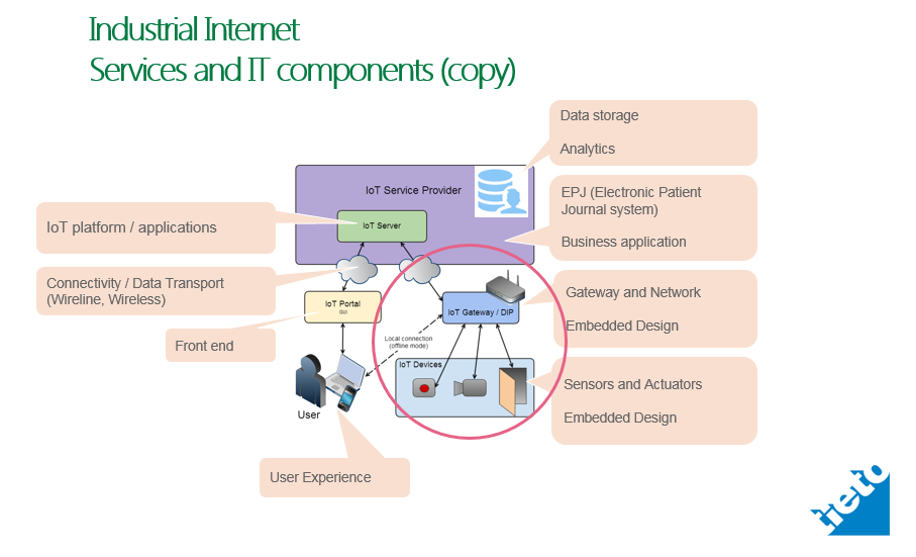
\includegraphics[width=0.9\textwidth]{layout}
	\label{fig:eSenseLayout}
	\caption{eSense Layout}
\end{figure}
\newpage

Examensarbetet bör innehålla följande
\begin{itemize}
	\item En utvärdering om mobilen är en möjlig och användbar lösning för både professionella vårdare men även för brukare av produkten.
	\item Finna referenscase och tillämpningar som finns eller borde finnas redan idag där multipla enheter ansluts till mobiltelefonen.
	\item Utvärdera fördelar och nackdelar med lösningen (mobilen som gateway eller router med anslutna medicinska enheter).
	\item Utvärdering av vilket OS som passar bäst för mobilen.
	\item Svara på frågan: Finns det open source lösningar som vi kan använda och vidareutveckla?\\
	\item Examensarbetet ska speciellt fokusera på
	\begin{itemize}
		\item Säkerhet. Här finns det många olika aspekter och vi bör fokusera på några utvalda områden.
		\item Mobilplattform och val av OS
		\item Integration av enheter för mätning av
		\begin{itemize}
			\item Blodtryck, Puls, Blodsocker och INR.
		\end{itemize}
		\item Utvärdering av Continua certifiering.
		\item Utvärdering av lagliga krav som ställs på lösningen.
		\begin{itemize}
			\item Säkerhet
			\item Sekretess
			\item PLU
		\end{itemize}
		\item Användningsområden på lösningen.
	\end{itemize}
	\item Målet är att utföra en implementation i valt OS som använder
	\begin{itemize}
		\item Continua certifierade enheter för medicinska mätvärden
		\item Mobiltelefon som gateway/router.
		\item Kopplar samman mätenheter med mobiltelefon via Bluetooth/Wifi för kortdistanskommunikation.
		\item Integrera mot eSense via mobilnätet.
		\item Använda några av mobiltelefonens sensorer för att komplettera lösningen (GPS-lokalisering, plötslig acceleration(fall),...)
		\item Visa data och användare i en enkel Lifecare all
	\end{itemize}
	\item WoW (Way of Working)
	\begin{itemize}
		\item Examensarbetaren kommer medverka i eSense-teamets dagliga SCRUM-möten.
		\item En i teamet kommer utses till huvudmentor men hela teamet kommer ta på sig rollen som mentorer.
	\end{itemize}
\end{itemize}

Målet med detta examensarbete är att det skall vara en E-uppsats då resultatet både kan användas praktist och att man för att göra detta måste se vilka lagliga och sociala aspekter som påverkas.
\end{document}